\subsection{GN2 Hyperparameter Optimisation}\label{chap-GN2Opt}
The state-of-the-art flavour tagger at ATLAS is, at the time of writing, built on the \gls{gn2} architecture. Naturally, fine-tuning the model is required to further improve the performance. Many studies are ongoing to deliver yet a stronger tagger than the \gls{gn2} version presented in this thesis. A non-exhaustive list of ongoing research directions includes: 
\begin{itemize}
  \item Optimising the track selection and the jet reconstruction type. Moving towards yet a looser selection and letting the network sift through a larger set of background tracks could deliver further gains in performance.
  \item The inclusion of neutral constituent information by using jets defined as \gls{ufo}. Tracks are reconstructed from hits in silicon trackers and vertex detectors. Such hits are only recorded for charged particles flying through the active regions of the sensors. This approach entirely misses neutral particles, such as neutrons, neutral pions and kaons, and neutrinos. All but the latter leave measurable energy deposits in the calorimeters. The \gls{ufo} jet definition combines track information with calorimeter topocluster objects. Studies are ongoing to add this information to the set of tracks. 
  \item The inclusion of leptonic information. 40\% of $b$-hadrons include either an $e$ or a $\mu$ in the jet cone \cite{Tanabashi:2018oca}. As seen with \gls{gn1}, the inclusion of leptonic information in the set of tracks leads to a significant performance increase. Studies are ongoing to build a finer lepton-information analyser within \gls{gn2}.
  \item Hadronic decays of $\tau$ are a major source of background for analyses focusing on $c$-jet tagging, due to their similar signatures. Including these leptons in the classification objective has been seen to deliver promising results in initial studies. 
  \item Finer output classes categorisation. Currently, the simple labelling scheme deployed combines topologies with significant differences. For example, purely hadronic and semi-leptonic decays of $b$-jets are both labelled $b$-jets. Adopting greater flexibility in the definition of classes allows the model to fully utilise the unique signature of each process. 
  \item Integrating further expert information into the design is known to deliver a great boost to performance. Studies are ongoing to upgrade the set of auxiliary tasks, in particular for secondary vertex fitting and reconstruction. A \gls{gn2} model able to reliably reconstruct this information would have a use case in the ATLAS experiment beyond heavy-flavour jet tagging while benefitting from improved performance for this essential task.  
\end{itemize}

These design considerations are paramount to producing a more efficient tagger. An equally essential endeavour is to fine-tune the architecture to extract the best performance from a chosen strategy. This section focuses on some initial studies to perform \gls{hpo} and network architecture search for \gls{gn2}. The essential challenge is that a test of a change to the hyperparameters or the model architecture requires fully retraining a \gls{gn2} model from scratch. This is a costly process, as a single epoch of \gls{gn2} training takes roughly $\sim$28 min on 2 NVIDIA A100 \glspl{gpu} each fed data by 20 \gls{cpu} on a 30 million jets dataset with batch size 2000 evenly split on the \glspl{gpu}. \gls{gn2} has many hyperparameters that should be optimised to deliver optimal performance, among which the most relevant are: initial $LR$, maximal $LR$, end $LR$, the weights of the 2 auxiliary tasks, the amount of weight decay, the batch size, and the floating numbers precision. Important architecture-level elements to be optimised are the embedding dimension (output of the initialiser and as input and output of each transformer encoder), the depth of the initialiser, the number of layers and heads in the transformer encoder, the size of the transformer output, the auxiliary tasks \gls{dnn}, the activation functions, and the specific loss functions and their class-weights used. \\

Complex network require hardware accelerators such as \glspl{gpu} to be effectively trained. In this respect, a promising area of development is being pursued by \gls{cern}, with the introduction of a KubeFlow-backed server hosted on \textit{ml.cern.ch} \cite{KubeFlowCern}. KubeFlow is an open-source framework built on Kubernetes to perform machine learning operations such as training, inference, deployment, and hyperparameter optimisation. The project aims to centralise some \gls{gpu} resources into a single cluster with datastorage, efficient I/O reading capabilities, and dedicated \gls{gpu} nodes. Katib, KubeFlow's dedicated \gls{hpo} workload, is a promising approach to perform effective hyperparameter optimisation with state-of-the-art autoML techniques to automate and refine the strategy to test and converge on the best hyperparameters \cite{george2020katib}. At the time of writing, the server is still in a beta phase with little hardware accessible, thereby removing it from consideration as a possible solution to carry out the full \gls{hpo} of \gls{gn2}. However, the \textsc{salt} framework used to train \gls{gn2} has been adapted to run on any KubeFlow platform, with initial tests showing promising possibilities for the Collaboration. Being accessible to any member of ATLAS, this project would ``democratise'' access to computing-intensive studies for institutes lacking an advanced \gls{hpc}. \\

Large \gls{nn} such as large language models that are being developed at ATLAS will require clusters designed for machine learning, with many \glspl{gpu} accessible on dedicated nodes. This paradigm of computing is markedly different from the typical grid-based distributed computing currently accessible to \gls{lhc} experiments. While \gls{mc}-based samples and sub-sampled datasets can be effectively processed by autonomous parallel jobs, \gls{ml} requires communication between the different jobs to keep the weights of the model synchronised on the different \glspl{gpu}. A fast connection between these \glspl{gpu} is essential, as is having fast read access to the full dataset. Distributing the computation across \glspl{hpc} that are geographically distant, as is common with the current \gls{cern} computing grid, is not effective for this purpose. The \gls{cern} KubeFlow server is a promising area of development for the future computational needs of ATLAS. Furthermore, having a framework compatible with KubeFlow allows operating on multiple platforms, giving the flexibility to scale resource access for computationally demanding tasks. Most private and public cloud providers, such as Google Cloud, Amazon Web Service, and Microsoft Azure, are KubeFlow-compatible and host a larger amount of state-of-the-art \glspl{gpu}. \textsc{Salt} can be effectively deployed on the infrastructure of these cloud providers or \gls{cern}'s KubeFlow server with no noticeable distinctions for the user. \\

While leveraging a large amount of computing power is a natural solution to the challenging task of \gls{hpo} of a ``large'' neural network by ATLAS standards, a more refined technique can be exploited in the present case. Recent works from the \gls{ml} community suggest that the optimal hyperparameters of a nominal model can be estimated from a smaller model \cite{yang2021tuning}. Here smaller refers to either the depth - the number of layers - or the width - the number of neurons per layer and, in the case of a transformer, also the number of heads in the multihead attention - of the neural network. Ref. \cite{pmlr-v139-yang21c} establishes the mathematical foundation backing this surprising behaviour of deep neural network: the \gls{mup}. The rest of this section is dedicated to introducing and defining the maximal update parametrisation before establishing its relevance for \gls{hpo}.

\subsubsection{Maximal Update Parametrisation}
The maximal update parametrisation is first and foremost a \textit{parametrisation}. In this context, the parametrisation of a neural network refers to the definition of the weights of each neuron, the way they are initialised, and how they are updated from a given optimisation algorithm, such as Adam or \gls{sgd} \cite{adamPaper}. The default or \textit{standard} parametrisation (SP) follows the so-called LeCun parametrisation \cite{LeCun2012}. This parametrisation, routinely deployed in \gls{ml} frameworks such as PyTorch \cite{pytorch}, initialises the weights by sampling them from a Gaussian or Uniform distribution with mean 0 and standard deviation given by the inverse of the input dimension of the layer the weight belongs to. For both Adam and \gls{sgd}, a single master learning rate (LR) $\eta$ is used for all weights. For \gls{mup}, some subtle differences are introduced, as summarised in Table~\ref{tab:mupvsspdef}. Mainly, the output layer weights are sampled from a Gaussian with a standard deviation being the inverse of the input dimension \textbf{squared} of the output layer. Concerning the learning rates, the hidden and output layers are scaled down by their respective input dimension for Adam. For \gls{sgd}, the output layer $LR$ is scaled similarly, but the input and the bias $LR$ are scaled up by the output dimension of these layers. 

\begin{table}[h]
  \begin{center}
      \begin{tabular}{c|cc|cc|cc} 
      	 \hline \hline
          & \multicolumn{2}{c|}{Initialisation Distribution} & \multicolumn{2}{c|}{Adam $LR$} & \multicolumn{2}{c}{SGD $LR$}  \\
            & $SP$  & \gls{mup} & $SP$  & \gls{mup} & $SP$  & \gls{mup}  \\ \hline
          $w^{L_\textrm{inp}}$ & $\sim$ $\mathcal{N}\left(0, \frac{1}{d^{\textrm{in}}_{L_\textrm{inp}}}\right)$ & $\sim$ $\mathcal{N}\left(0, \frac{1}{d^{\textrm{in}}_{L_\textrm{inp}}}\right)$                                         & $\eta$ & $\eta$                                    & $\eta$ & $\eta \boldsymbol{\times d^{\textrm{out}}_{L_\textrm{inp}}}$ \\ 
          $w^{L_\textrm{hid}}$ & $\sim$ $\mathcal{N}\left(0, \frac{1}{d^{\textrm{in}}_{L_\textrm{hid}}}\right)$ & $\sim$ $\mathcal{N}\left(0, \frac{1}{d^{\textrm{in}}_{L_\textrm{hid}}}\right)$                                         & $\eta$ & $\eta \boldsymbol{/ d^{\textrm{in}}_{L_\textrm{hid}}}$ & $\eta$ & $\eta$                                    \\ 
          $w^{L_\textrm{out}}$ & $\sim$ $\mathcal{N}\left(0, \frac{1}{d^{\textrm{in}}_{L_\textrm{out}}}\right)$ & $\sim$ $\mathcal{N}\left(0, \frac{1}{d^{\textrm{in}}_{L_\textrm{out}}\times \boldsymbol{d^{\textrm{in}}_{L_\textrm{out}}}}\right)$  & $\eta$ & $\eta \boldsymbol{/ d^{\textrm{in}}_{L_\textrm{out}}}$ & $\eta$ & $\eta \boldsymbol{/ d^{\textrm{in}}_{L_\textrm{out}}}$ \\
          $b^{L} \;\forall L$ & 0 & 0                                                                                                                                                                                          & $\eta$ & $\eta$                                    & $\eta$ & $\eta \boldsymbol{\times d^{\textrm{out}}_{L}}$              \\  \hline \hline
      \end{tabular}
    \caption{Comparing the Standard Parametrisation (SP) to the Maximal Update Parametrisation ($\mu P$), as defined in Ref. \cite{yang2021tuning} based on the work of Ref. \cite{pmlr-v139-yang21c}.}
    \label{tab:mupvsspdef}
  \end{center}
\end{table}

This particular derivation of \gls{mup}, taken from Ref. \cite{yang2021tuning}, is equivalent to the original \gls{mup} derivation introduced in Ref. \cite{pmlr-v139-yang21c}. \gls{mup} turns out to be the unique parametrisation that maximally updates the weights of a neural network. The updates are ``\textit{maximal}'' in the sense that they are as large as they could be for a given LR to avoid any instabilities. For the specific case of the attention mechanism computed by the multi-head attention of transformers, the scaling has to be modified from $\sqrt{d_k} \rightarrow d_k$ to properly scale with width \cite{yang2021tuning}. Figure~\ref{fig:muspweights} shows a comparison of the size of the pre-activation of a \gls{gn2} model with \gls{mup} parametrisation to a standardly parametrised \gls{gn2}, referred to as the $SP$ model, at different training steps. Each curve displays, for different embedding widths in the transformer and the track initialiser, the sum of the absolute values of the weights before the activation ($L_1(\textrm{layer}) = \sum_{w_i \in \textrm{layer}} |w_i|$) for the initialiser and transformer models only. Three timesteps are displayed for each model, the initialisation ($t=1$) and after 1 ($t=2$) and 2 ($t=2$) training steps. The interesting behaviour highlighted in this figure is that for the $SP$ model, the pre-activation weights blow up with width during training as shown by the exponential rise of the sum of pre-activations. For \gls{mup} however, the $L_1$ of each layer stays flat with width even during training, proving the correct parametrisation of the model and the ``width-independent'' scaling. This unstable behaviour of the $SP$ parametrisation is easily highlighted thanks to the use of a large and fixed learning rate (here $LR = 10^{-2}$). 

\begin{figure}[h!]
  \centering
  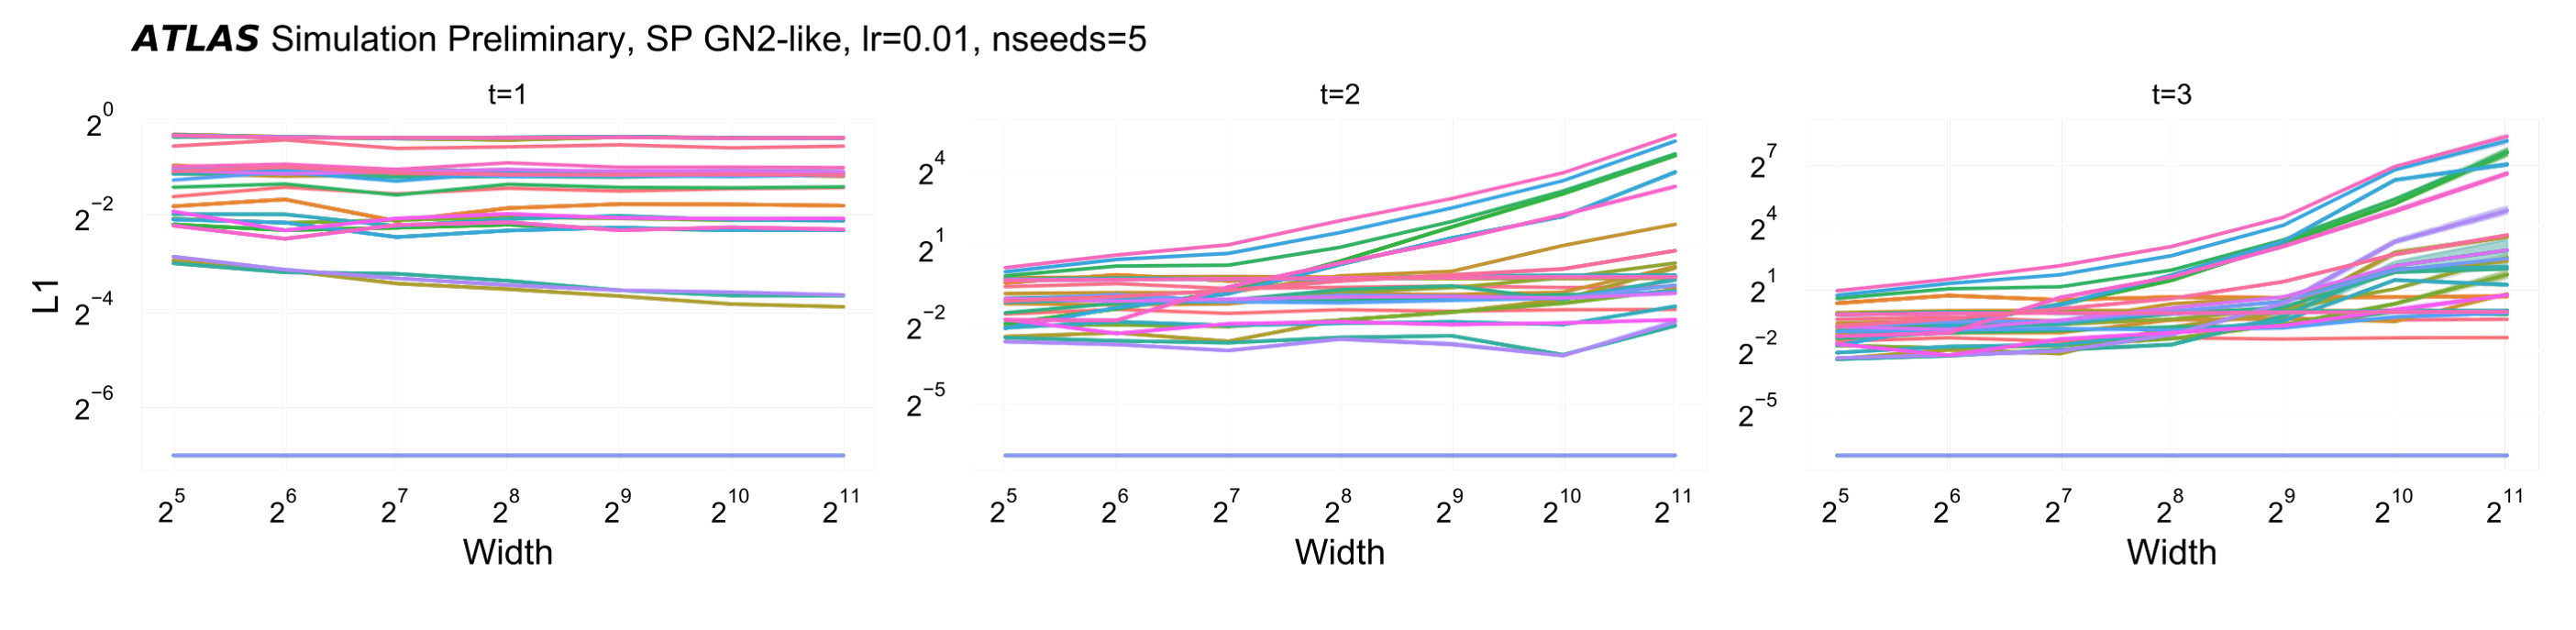
\includegraphics[width=\textwidth]{Images/FTAG/GN/HPO/spweights.png}\\
  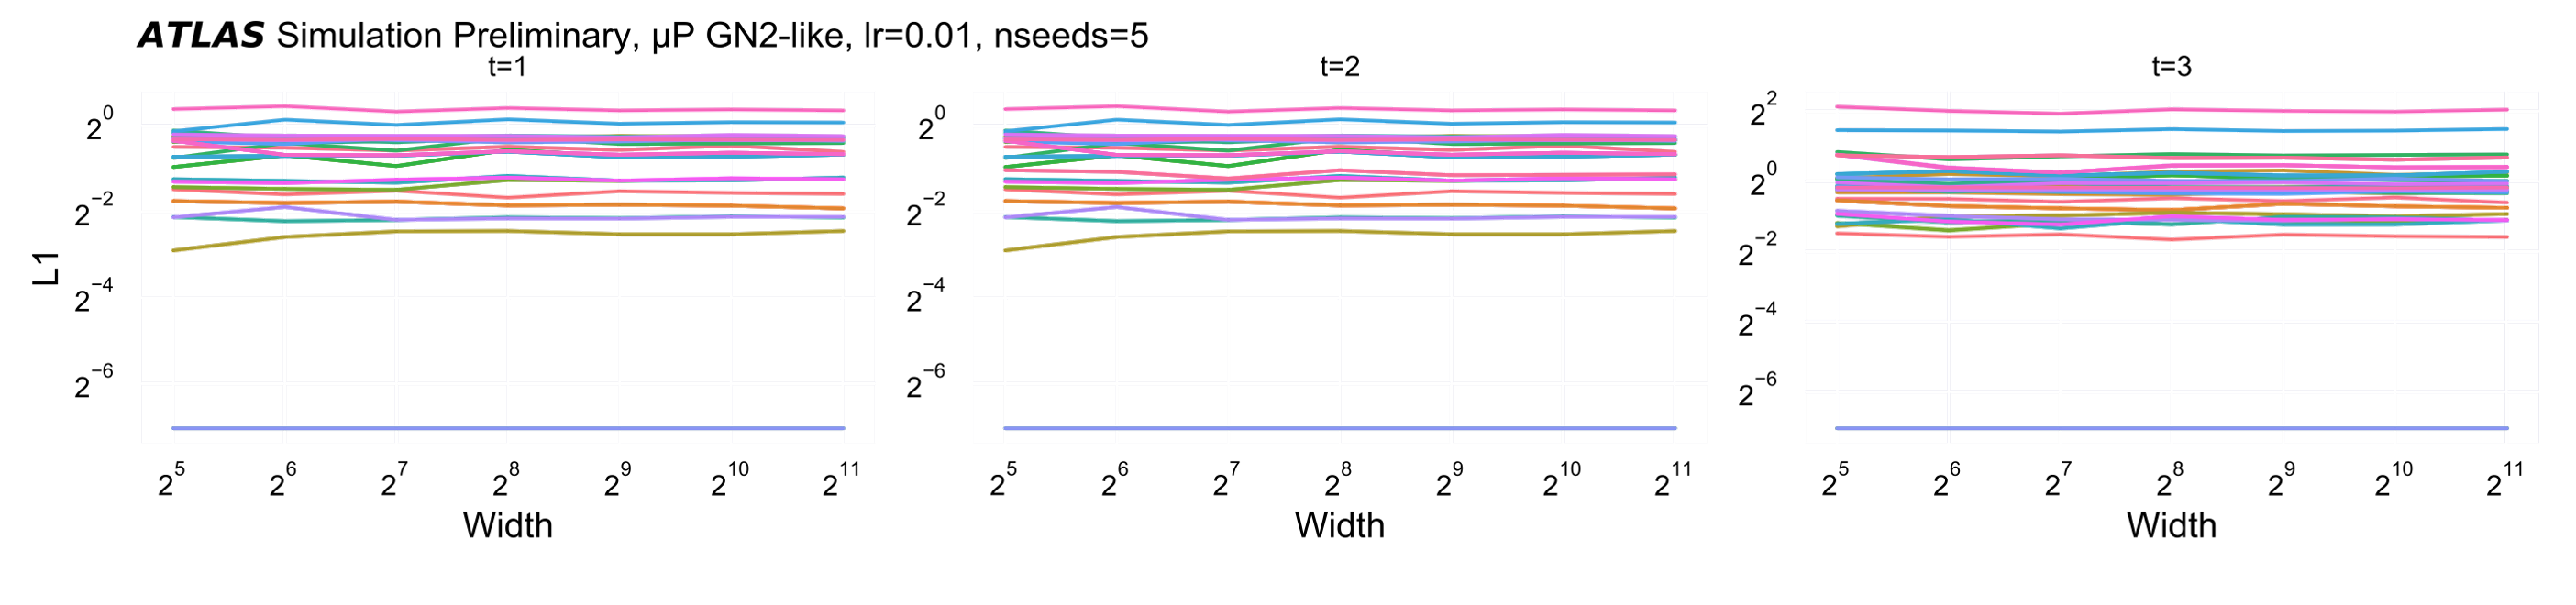
\includegraphics[width=\textwidth]{Images/FTAG/GN/HPO/mupweights.png}
  \caption{The sum of the absolute values of the pre-activation weights for the different layers in the initialiser and transformer parts of a GN2-like model in standard parametrisation ($SP$ - top) and in $\mu$P parametrisation (bottom), at three timesteps: initialisation ($t=1$ - left), after one training step with $LR = 10^{-2}$ ($t=2$ - centre), and a second training step ($t=3$) \cite{publicplotMUP}. The models displayed are labelled GN2-like as they lack auxiliary tasks.}
  \label{fig:muspweights}
\end{figure} 

\paragraph{}Theoretically, a \gls{mup} model should deliver equal to better performance to an equivalent $SP$ model when both have optimal hyperparameters. This behaviour is due to the maximal updating of the former, leading to optimal in-depth updates of all layers. The standard parametrisation does not implement this correct updating, with outer layers closer to the loss function having an opacity effect on the propagation of the update for the input layers proportionally to their widths. Scaling down the learning rate is not a sufficient modification to correct the SP: as displayed in Figure~\ref{fig:muspweights}, not all layers update incorrectly with some pre-activation sum staying flat across the widths. By updating all activation maximally independently of the width, \gls{mup} outperforms $SP$ for a tuned learning rate \cite{pmlr-v139-yang21c}. A significant advantage of this parametrisation is that the optimal learning rate for a \gls{mup} architecture becomes width-independent. This leads to the $\mu$Transfer algorithm for \gls{hpo}, where the best hyperparameters for a \gls{mup} model are found on a version with fewer neurons per layer (smaller width) and the found optimal ones are transferred to the full-size model at no extra cost (0-shot transferred) \cite{yang2021tuning}. The benefits of adopting the maximal update parametrisation are:
\begin{enumerate}
  \item Better performance of a \gls{mup} model compared to an $SP$ model for a tuned learning rate.
  \item Improved hyperparameter optimisation with the $\mu$Transfer algorithm: performing the \gls{hpo} scan on a smaller and easier-to-train model to directly gives the best set of hyperparameters to the full-size models (\textit{0-shot transfer}). 
  \item Better hardware usage for \gls{hpo}: a smaller model can be trained on a single \gls{gpu}. This is of particular interest for the ATLAS Collaboration, as most of the \gls{gpu} resources accessible are scattered through geographically distant computing sites.  
  \item Simplified architecture: with \gls{mup}, a wider model outperforms a smaller model if no overtraining occurs. Therefore, the best learning rate hyperparameter has to be found once for all \gls{gn2} models of varying widths and the widths are chosen based on the desired computational complexity.
\end{enumerate}

Hyperparameters that can be optimised with the $\mu$Transfer algorithms are said to be $\mu$Transferable. They consist of \cite{yang2021tuning}: 
\begin{itemize}
  \item Learning rate and parameters of a learning rate scheduler.
  \item Optimiser parameters, such as the momentum, and the Adam $\alpha$ and $\beta$.
  \item Initialisation parameters, such as the initial per layer variances.
  \item Multiplicative constants.
\end{itemize}
Unfortunately, many parameters do not $\mu$Tranfer as they combine aspects of the model and the data, and must be studied on the full-size model directly. For example, the regularisation parameters (dropout, weight decay, normalisation, ...) do not scale, as a particular model size will overfit depending on the data. Finally, the last important family of hyperparameters are those defining the scale of the problem. These parameters are not found from $\mu$Transfer but rather ``$\mu$Transfered along''. They consist of the width\footnote{Number of neurons per layer, number of attention heads in a transformer, ...}, the depth, and the batch size. Only the scaling along width is theoretically proven thanks to \gls{mup}, while the others are empirically observed to hold \cite{yang2021tuning}.\\

Studies of the \gls{mup} parametrisation and the $\mu$Transfer algorithm have been performed for the \gls{gn2} flavour tagger. In this architecture, the most relevant dimensions are the width and the depth of the transformer part, tasks with building a conditional representation of the tracks from the embedded tracks processed by the initialiser network. These two dimensions are keys as most of the parameters of the \gls{gn2} model are in the transformer and the initialiser, with only a few parameters set in the networks of the primary and auxiliary tasks. As such, the chosen dimension to scale with $\mu$Transfer is the embedding width. The number of parameters in the transformer associated with the embedding width scales quadratically with this parameter, making it the most sensitive dimension to define the complexity of \gls{gn2}. 

\begin{figure}[h!]
  \centering
  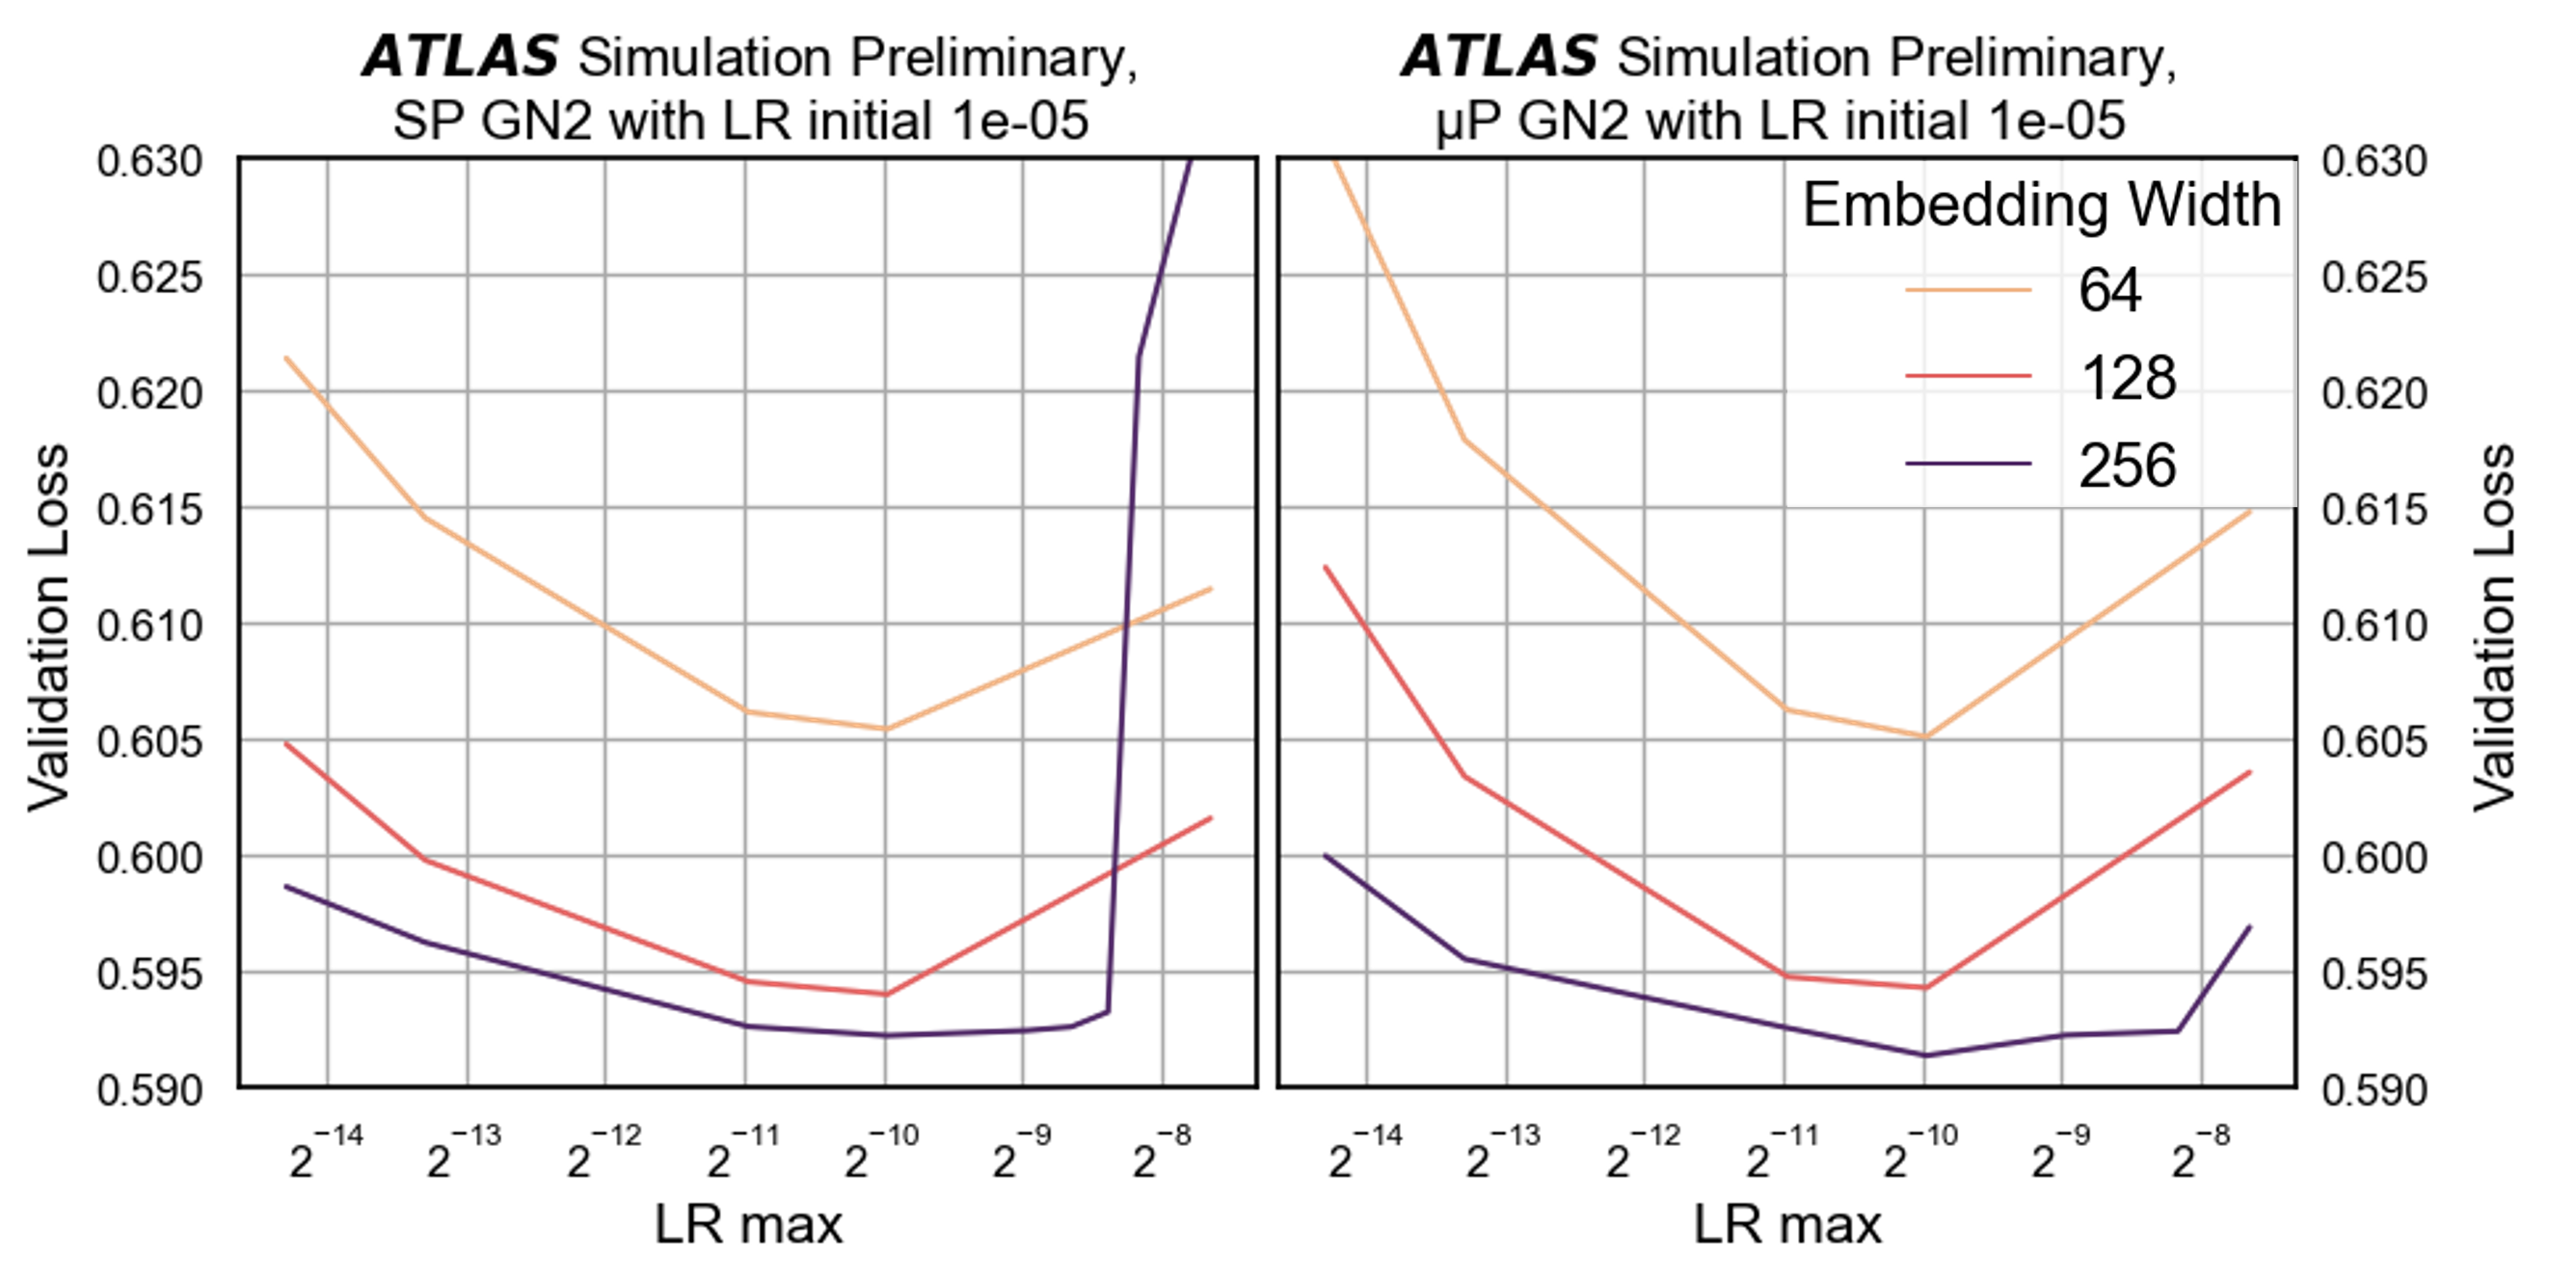
\includegraphics[width=\textwidth]{Images/FTAG/GN/HPO/maincompmupsp.png}
  \caption{Comparison of a maximal learning rate value scan at an initial learning rate value of $10^{-5}$ for an $SP$ (left) and a \gls{mup} GN2 models (right) for three different embedding widths: 64 (yellow), 128 (red), and 256 (purple) \cite{publicplotMUP}. The $y$-axis displays the validation loss attained.}
  \label{fig:maincompmupsp}
\end{figure} 

\paragraph{}To demonstrate the effect of \gls{mup} on \gls{gn2}, a hyperparameter optimisation campaign of the initial and maximal value of the learning rate\footnote{The final value, an LR end of $10^{-5}$, is kept fixed in all tests due to the limited compute available.} is performed using the standard and maximal update parameterisation, $SP$ vs \gls{mup}. Three embedding widths are considered: the nominal 256, defining a \gls{gn2} model with 2.3M parameters, a mid-size 128 width with 0.72M parameters, and a small 64 width model with 0.23M parameters. Interestingly, this smaller model with an embedding width 1/4 of the full model only has a 1/10 of the parameters. Furthermore, the small model is trainable on a single \gls{gpu} while the full and mid-size models required two \glspl{gpu} to be trained in a reasonable amount of time. All models are full \gls{gn2} models trained on 30M PFlow jets\footnote{Composed of 60\% $t\bar{t}$ and 40\% $Z'$.} for 40 epochs with batch size 1024. Parameters not mentioned are kept similar between embedding widths and parametrisations, and the epoch giving the lowest validation loss is chosen from each run. Figure~\ref{fig:maincompmupsp} outlines the main result of this study, displaying the various $LR$ max considered at the best $LR$ initial found ($10^{-5}$). Three main observations are drawn from these results:
\begin{enumerate}
  \item With \gls{mup}, the wider \gls{gn2} models - larger embedding width - always outperform the smaller versions. 
  \item Wider models do not always outperform smaller models with SP. In particular, at large LR max, the wider model becomes unstable and its performance in terms of validation loss significantly decreases.
  \item The optimal LR max (and LR init as shown in Figure~\ref{fig:fullSPmup}) are shared across widths with \gls{mup}, while no such behaviour is guaranteed for $SP$ - but is observed in the present case.
\end{enumerate}

\begin{figure}[h!]
  \centering
  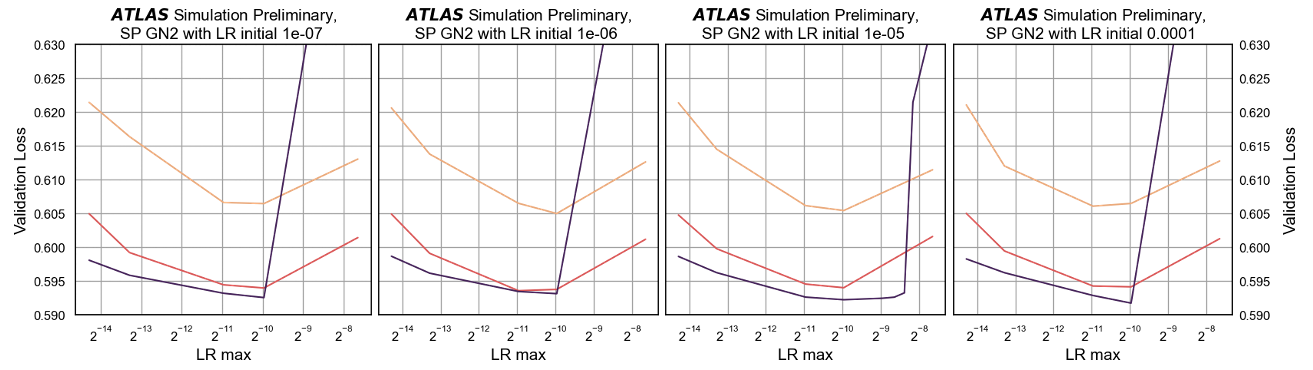
\includegraphics[width=\textwidth]{Images/FTAG/GN/HPO/fullSP2.png}\\
  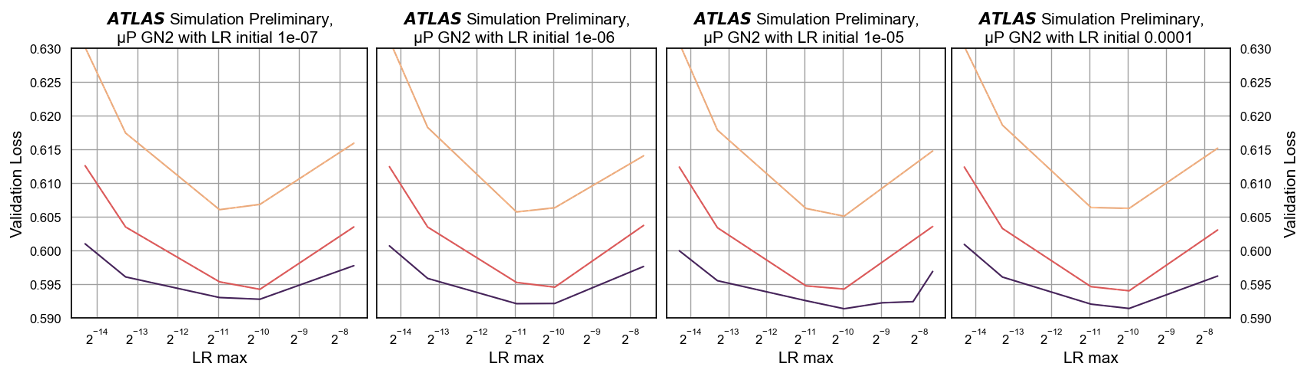
\includegraphics[width=\textwidth]{Images/FTAG/GN/HPO/fullmup2.png}
  \caption{Scan of the maximal learning rate ($x$-axis) versus initial learning rate (individual column) as measured by the validation loss ($y$-axis) of $SP$ models (top) and the $\mu$P model (bottom) with three different embedding widths: 64 (yellow), 128 (red), and 256 (purple) \cite{publicplotMUP}. The scan at LR initial = $10^{-5}$ benefitted from more tests to capture the sudden rise in validation loss at larger LR max for SP.}
  \label{fig:fullSPmup}
\end{figure} 

The full LR init vs LR max scans can be found in Figure~\ref{fig:fullSPmup} for $SP$ and \gls{mup}. Changing the LR init has little effect on the reached performance, due to the LR scheduler quickly moving away from the initial value and the common LR end value of $10^{-5}$ shared by all models at the end of training. The LR max however is a significant hyperparameter having a large impact on performance. All $SP$ models with 256 embedding widths are found to become unstable at large values of max LR. Note that the scan at LR initial = $10^{-5}$ benefitted from more tests to capture the sudden rise in validation loss at larger LR max. As expected from the previous discussion, all \gls{mup} models stay stable, even at larger values of the learning rate. On the contrary, $SP$ models become unstable with large LR max. \gls{mup} models share the same optimal LR parameters, although some variance impacts the precision of the method on the smallest model. Due to the limited computing power available, only one seed was run per test, introducing some unmeasured statistical variance in the output. An essential conclusion in this respect is the computing gain from performing the \gls{hpo} on the smaller width model than the full-width one:
\begin{itemize}
  \item The full-width model (embedding size 256) has 2.3M parameters, taking $\sim$39 min per epoch on 2 A100 \glspl{gpu} each fed data by 20 \glspl{cpu}.
  \item The small-width model (embedding size 64) has 0.23M parameters, taking $\sim$20 min per epoch on 1 A100 \gls{gpu} fed data by 20 \glspl{cpu}.
\end{itemize}
Essentially, a single full-width model hyperparameter test is in computing terms equivalent to running 4 individual tests on the smaller model. Given a fixed computing budget, one can therefore have a far better coverage of the hyperparameter search space with $\mu$Transfer.\\

This optimisation study was carried out to demonstrate the benefits of \gls{mup} on \gls{gn2}. Interestingly, the optimal value found for both the \gls{mup} and $SP$ models is at an LR max = $5 \times 10^{-4}$ and LR initial = $10^{-5}$. The default values used in the prior training of \gls{gn2} were, by luck, the same LR max but a larger LR init of $10^{-7}$. To quantify the effect on performance, the $b$-efficiency versus $c$- and light-rejection on $t\bar{t}$ and $Z'$ of two \gls{mup} models are displayed in Figure~\ref{fig:rocmupGN2}, with the suboptimal one being the worst performing full-width model (LR max = $5 \times 10^{-5}$, LR init = $10^{-7}$) and the optimal one the best performing one (LR max = $5\times 10^{-5}$, LR init = $10^{-5}$). While the optimal and suboptimal models had close validation loss, respectively 0.601 and 0.591, a significant difference in background rejection at all efficiencies is observed. At a $b$-tagging \gls{wp} of 70\%, the suboptimal \gls{gn2} model underperforms the optimal one on $t\bar{t}$ by 18\% (14\%) on $c$-rejection (light-rejection) and the disparity is even higher on $Z'$, rising to 24\% (26\%) at a $b$-tagging \gls{wp} of 30\% - which is equivalent to the 30\% \gls{wp} on $t\bar{t}$.

\begin{center}
  \begin{figure}[h!]
  \centerline{
  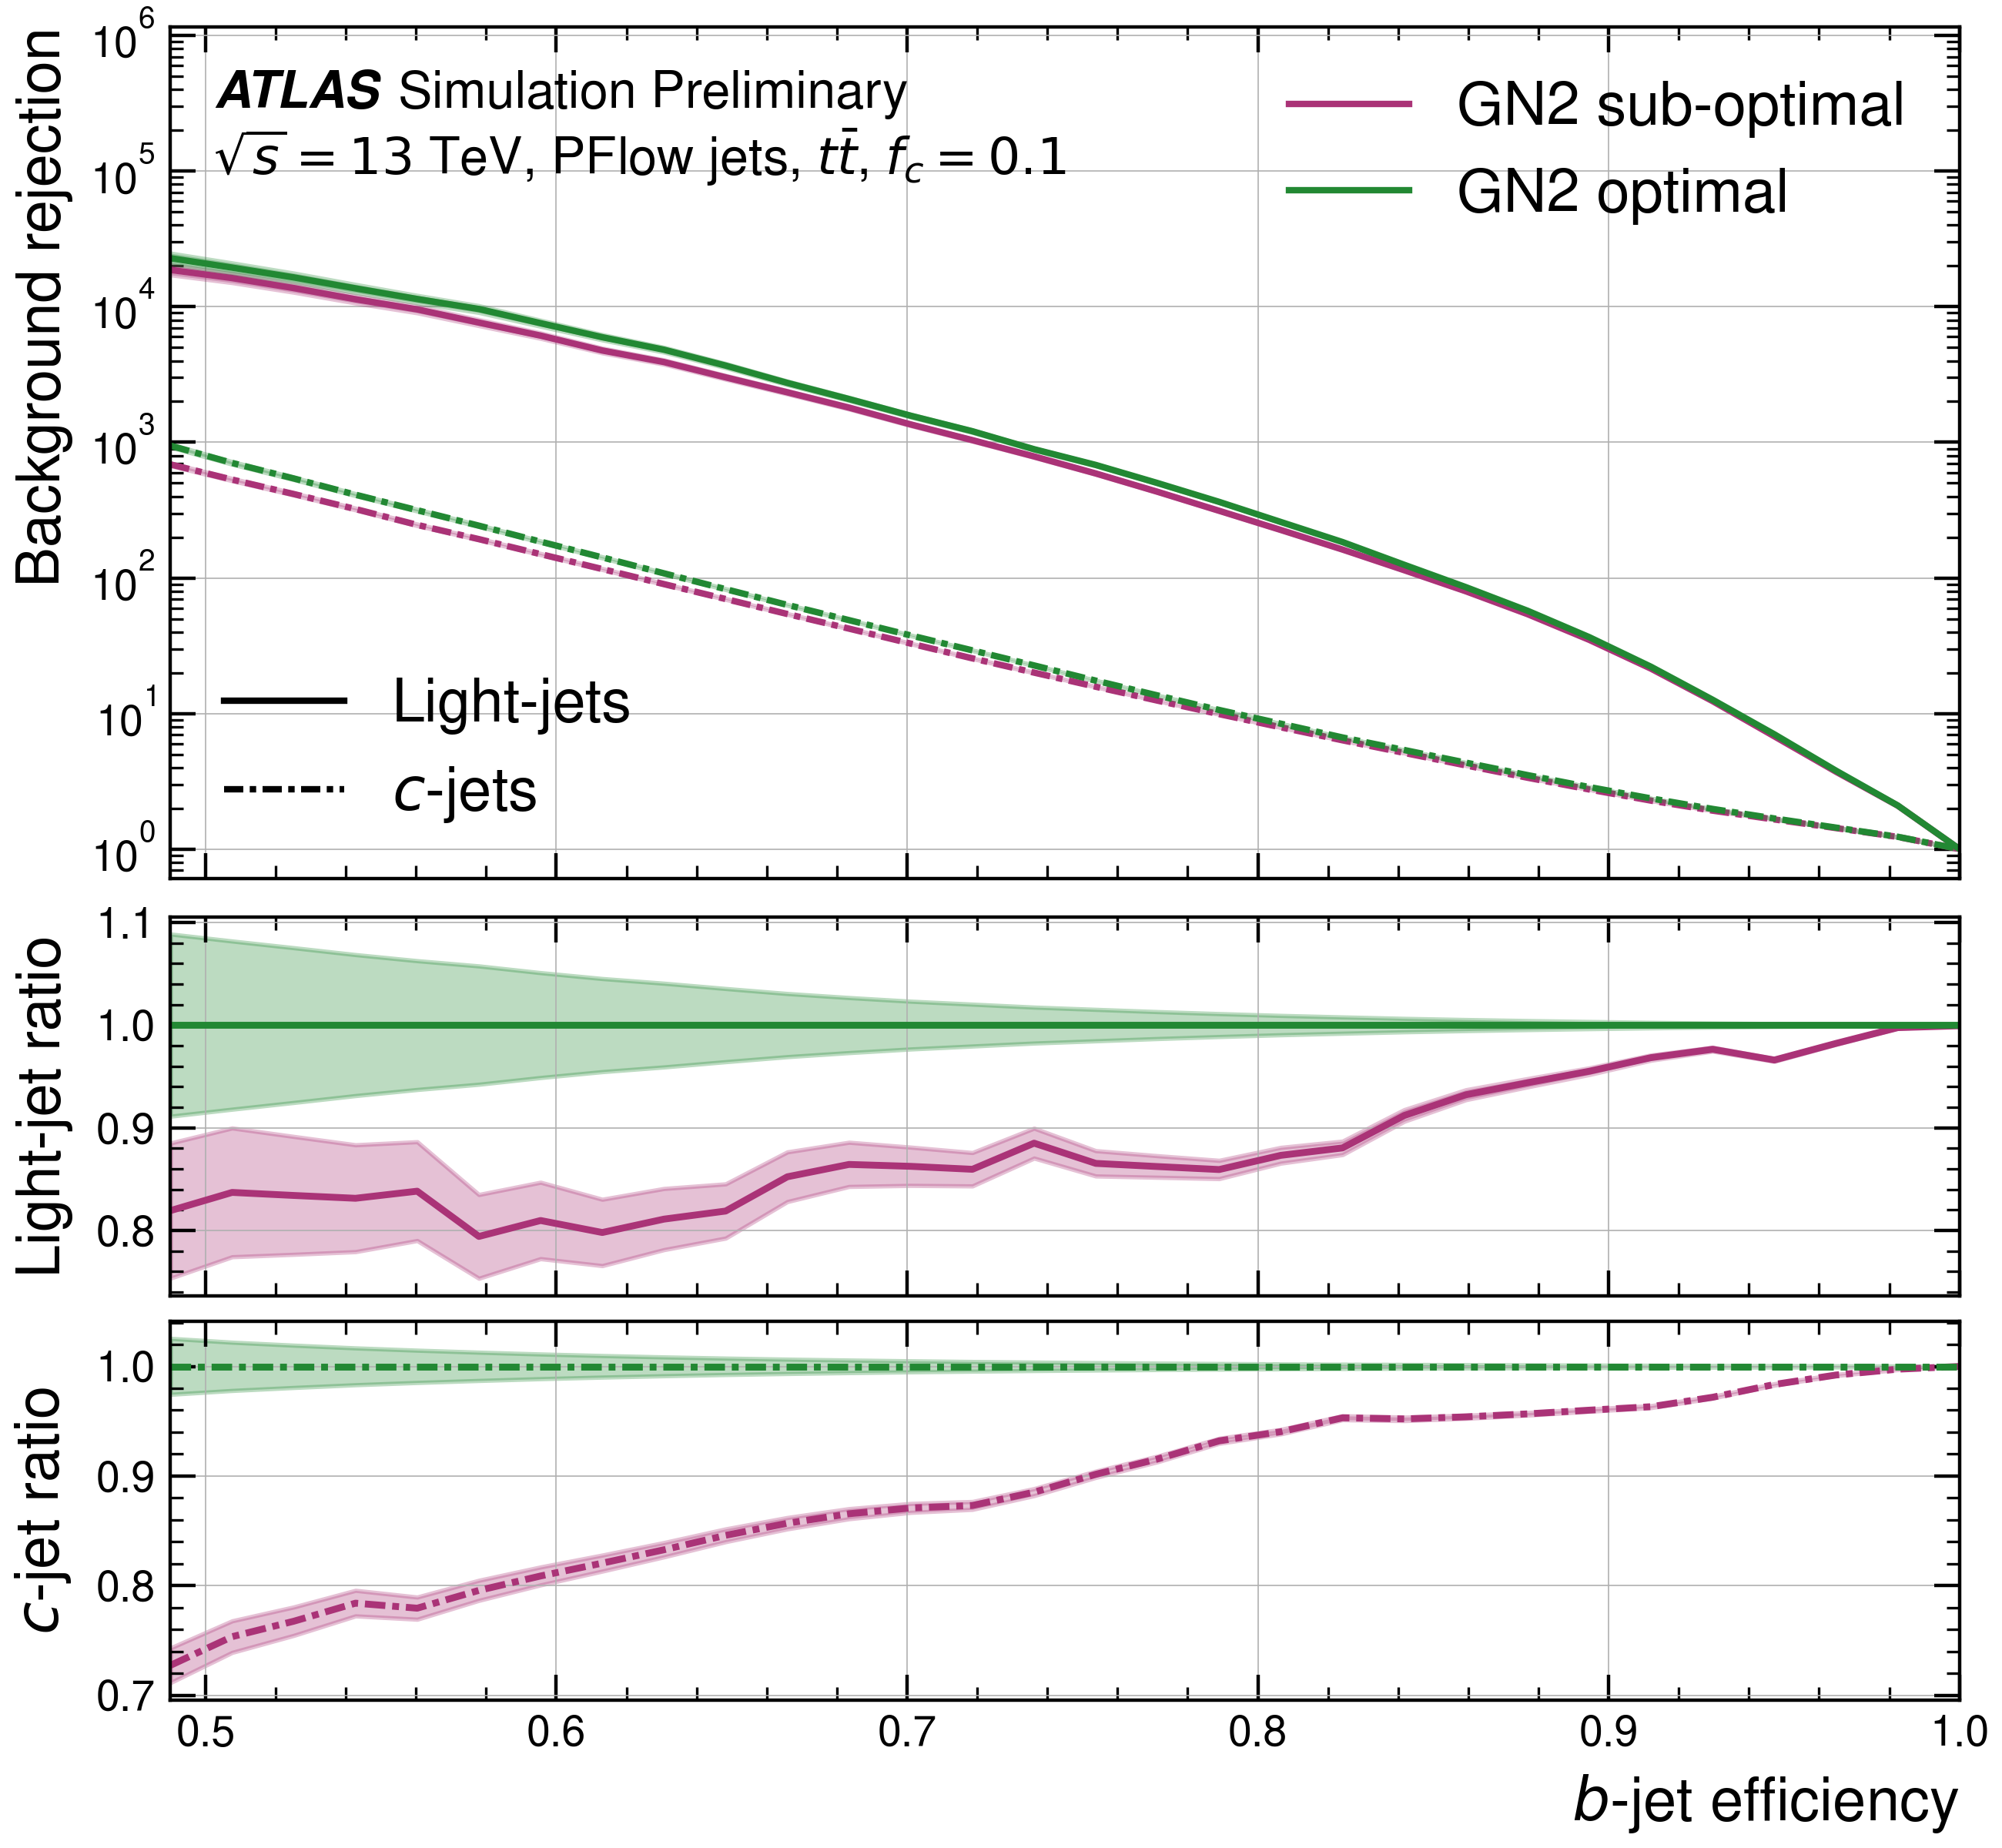
\includegraphics[width=0.50\textwidth]{Images/FTAG/GN/HPO/thesis_roc/roc_ttbar.png}
  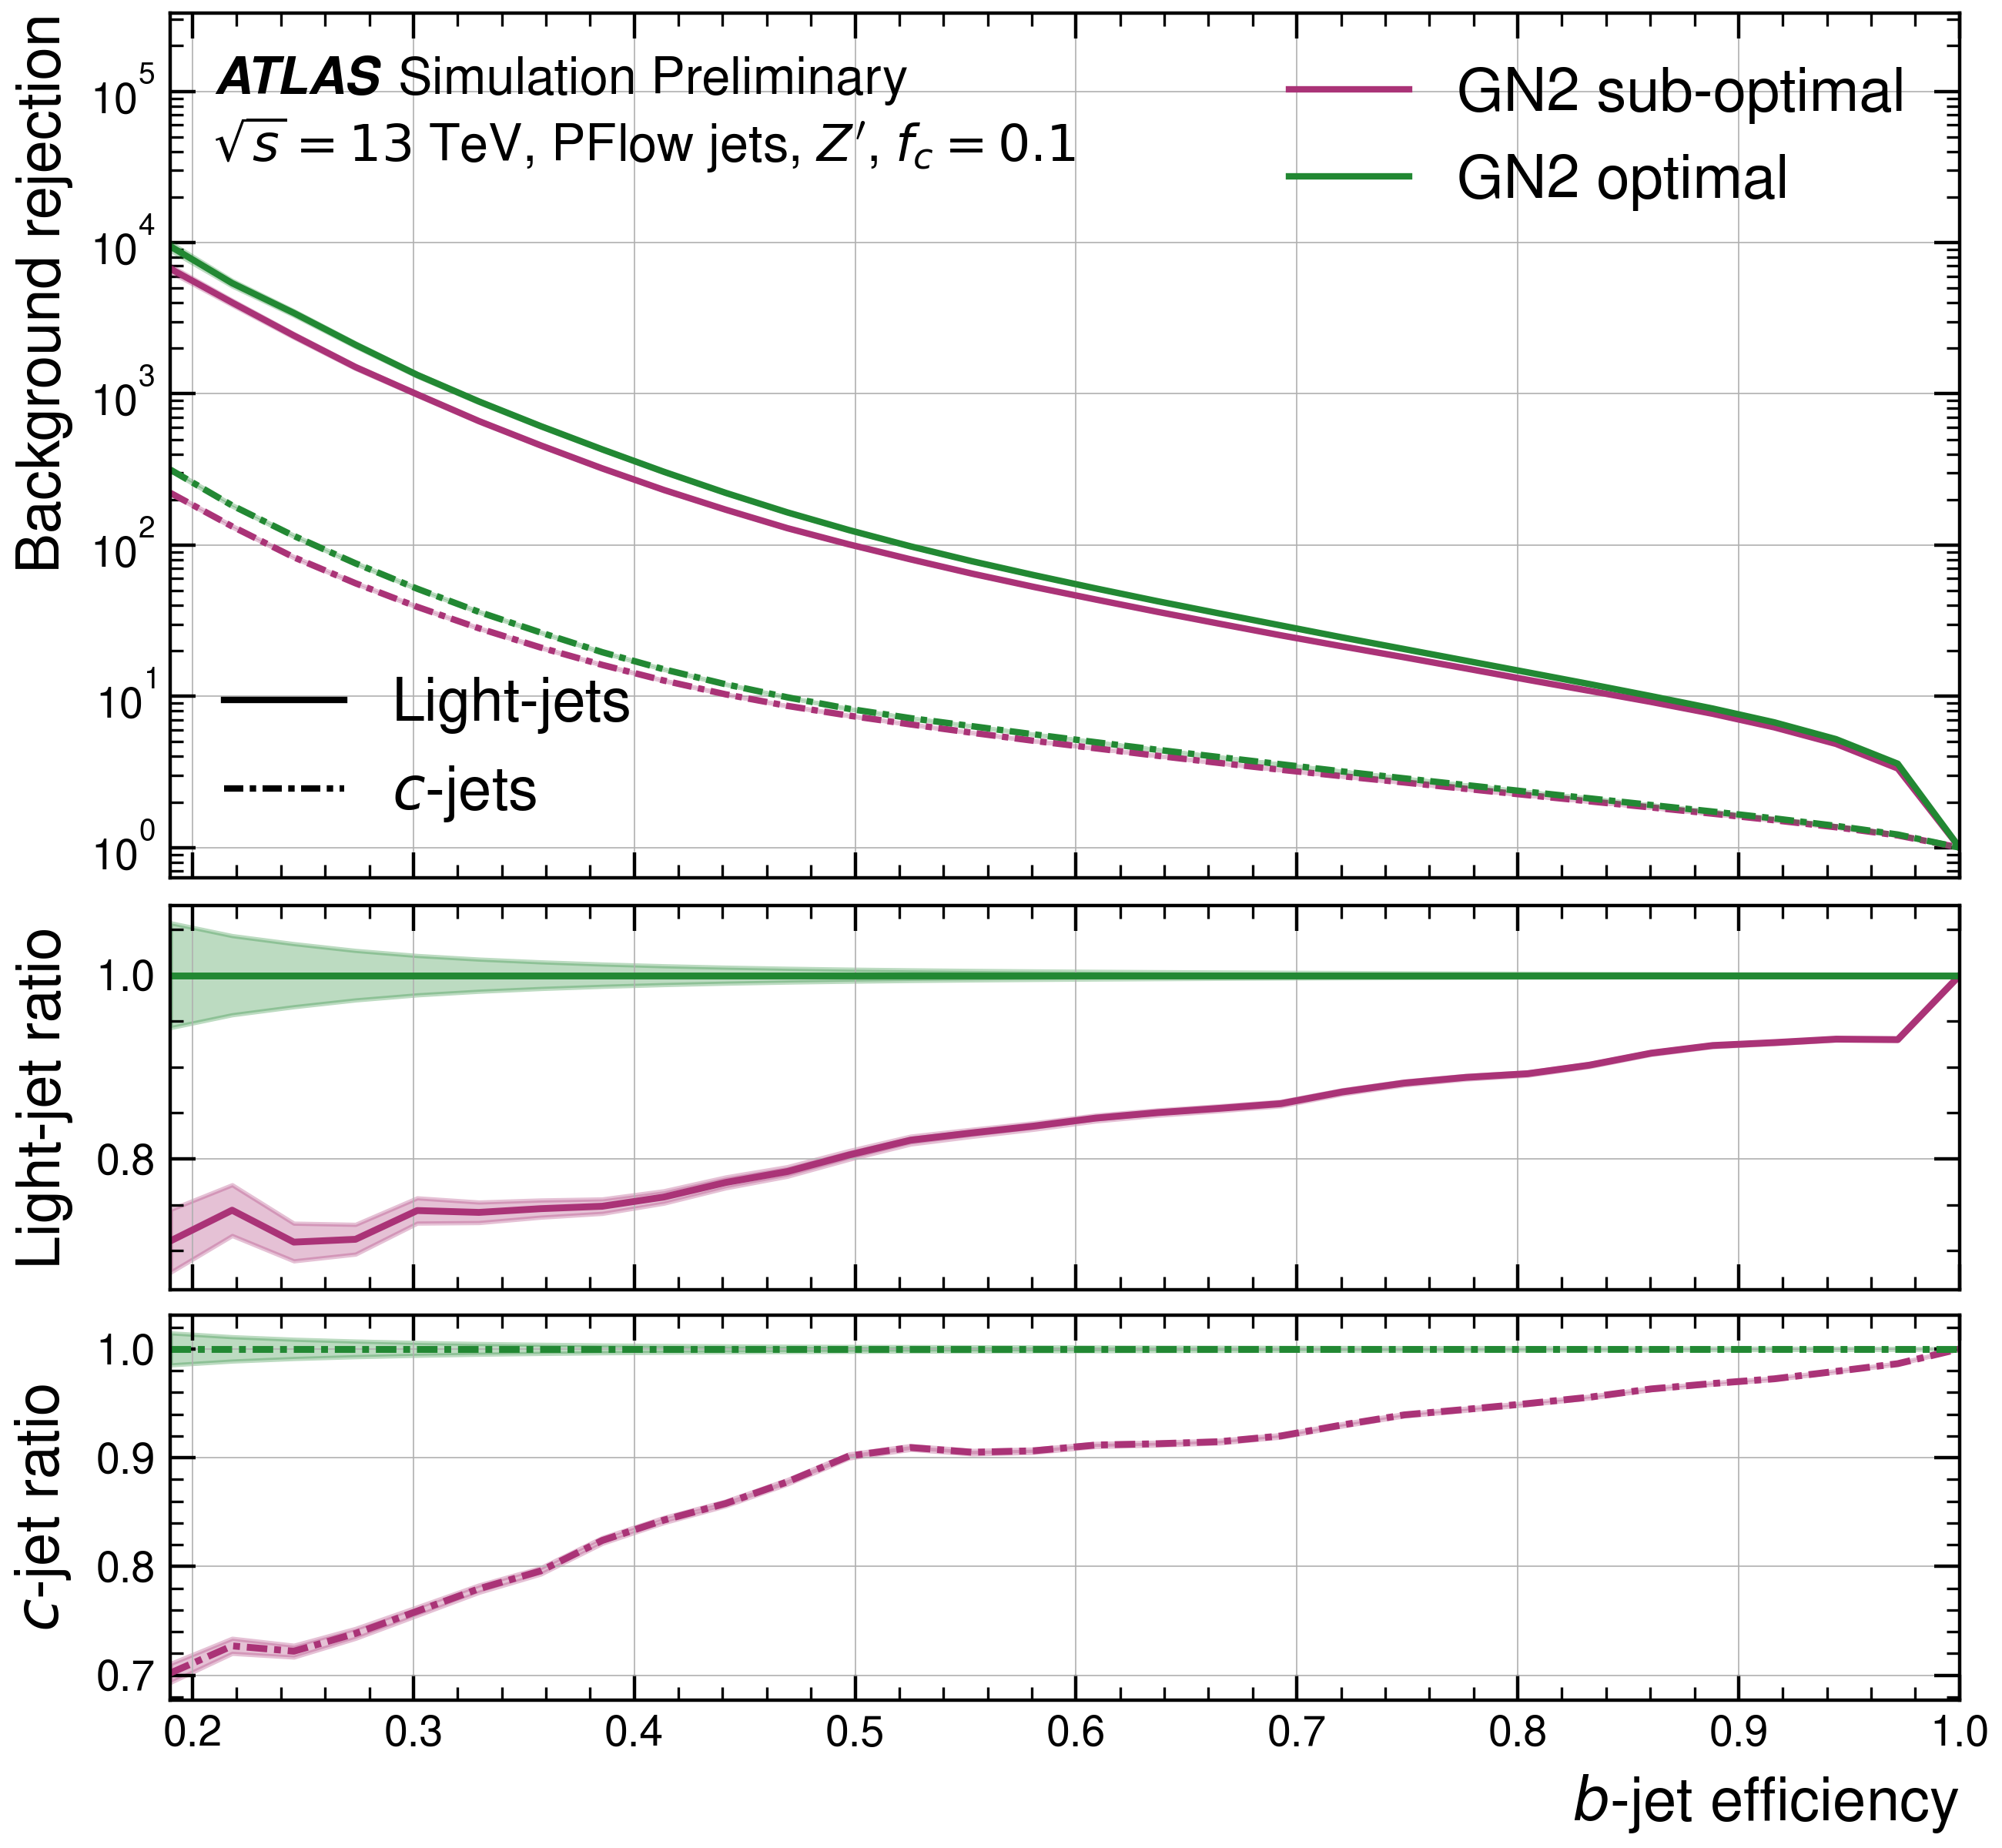
\includegraphics[width=0.50\textwidth]{Images/FTAG/GN/HPO/thesis_roc/roc_zp.png}
  }
  \caption{The $c$- and light-rejections as a function of the $b$-jet tagging efficiency in the $t\bar{t}$ (left) and $Z'$ (right) test samples \cite{publicplotMUP}. Models compared are the optimal $\mu$P GN2 (LR max = $5\times 10^{-5}$, LR init = $10^{-5}$) and the suboptimal $\mu$P GN2 (LR max $5 \times 10^{-5}$, LR init $10^{-7}$), all with 256 embedding width. Shaded regions represent the binominal error band.}
  \label{fig:rocmupGN2}
  \end{figure}
\end{center}

Additional tests of \gls{mup} performed with \gls{gn2} showed a similar correct scaling across depth with similar optimal hyperparameters being transferrable, as expected from empirical results \cite{yang2021tuning}. Due to the limited computing power available, the study of $SP$ versus \gls{mup} only encompassed two hyperparameters: the initial and maximal learning rate. The validity of the method has been confirmed and future studies optimising all the learning rate scheduler hyperparameters (including the warm-up and the learning rate at the end) will be carried out. Other hyperparameters that can best optimised with $\mu$Transfer are the initialisation variances of the different layers and the auxiliary objectives individual weights of Equation \ref{eq:totalobjgn}. \\

To summarise this section on \gls{hpo}, the present work introduces two approaches that are combined to deliver an improved hyperparameter optimisation:
\begin{itemize}
  \item Executing the \gls{hpo} on KubeFlow with the Katib workload to benefit from state-of-the-art autoML algorithm.
  \item Leveraging the \gls{mup} parametrisation to increase the performance of the tuned \gls{gn2} and benefit from the factor 4 boost in hyperparameter test coverage from $\mu$Transfer.
\end{itemize}
The full optimisation of \gls{gn2} is, at the time of writing, an ongoing effort of the ATLAS Collaboration.

\section{Calibration}\label{chap-calibration}
All flavour taggers presented in this chapter are trained on \gls{mc}-simulated events, as described in Section \ref{ftagdatasets}. As such, they depend on and acquire specific features of the simulated data that might not be present in the real data collected by the ATLAS experiment. While the Collaboration aims to generate the highest-fidelity simulations possible thanks to advanced software built on GEANT4 \cite{Agostinelli:602040} and many other specialised frameworks, inherent and unavoidable differences are left. To quantify the effect of using a simulation-trained network on real data, the ATLAS Collaboration performs Data-Monte Carlo agreement and calibration studies, as suggested in Figure~\ref{fig:calibFtagDL1d}.

\begin{center}
  \begin{figure}[h!]
  \centerline{
  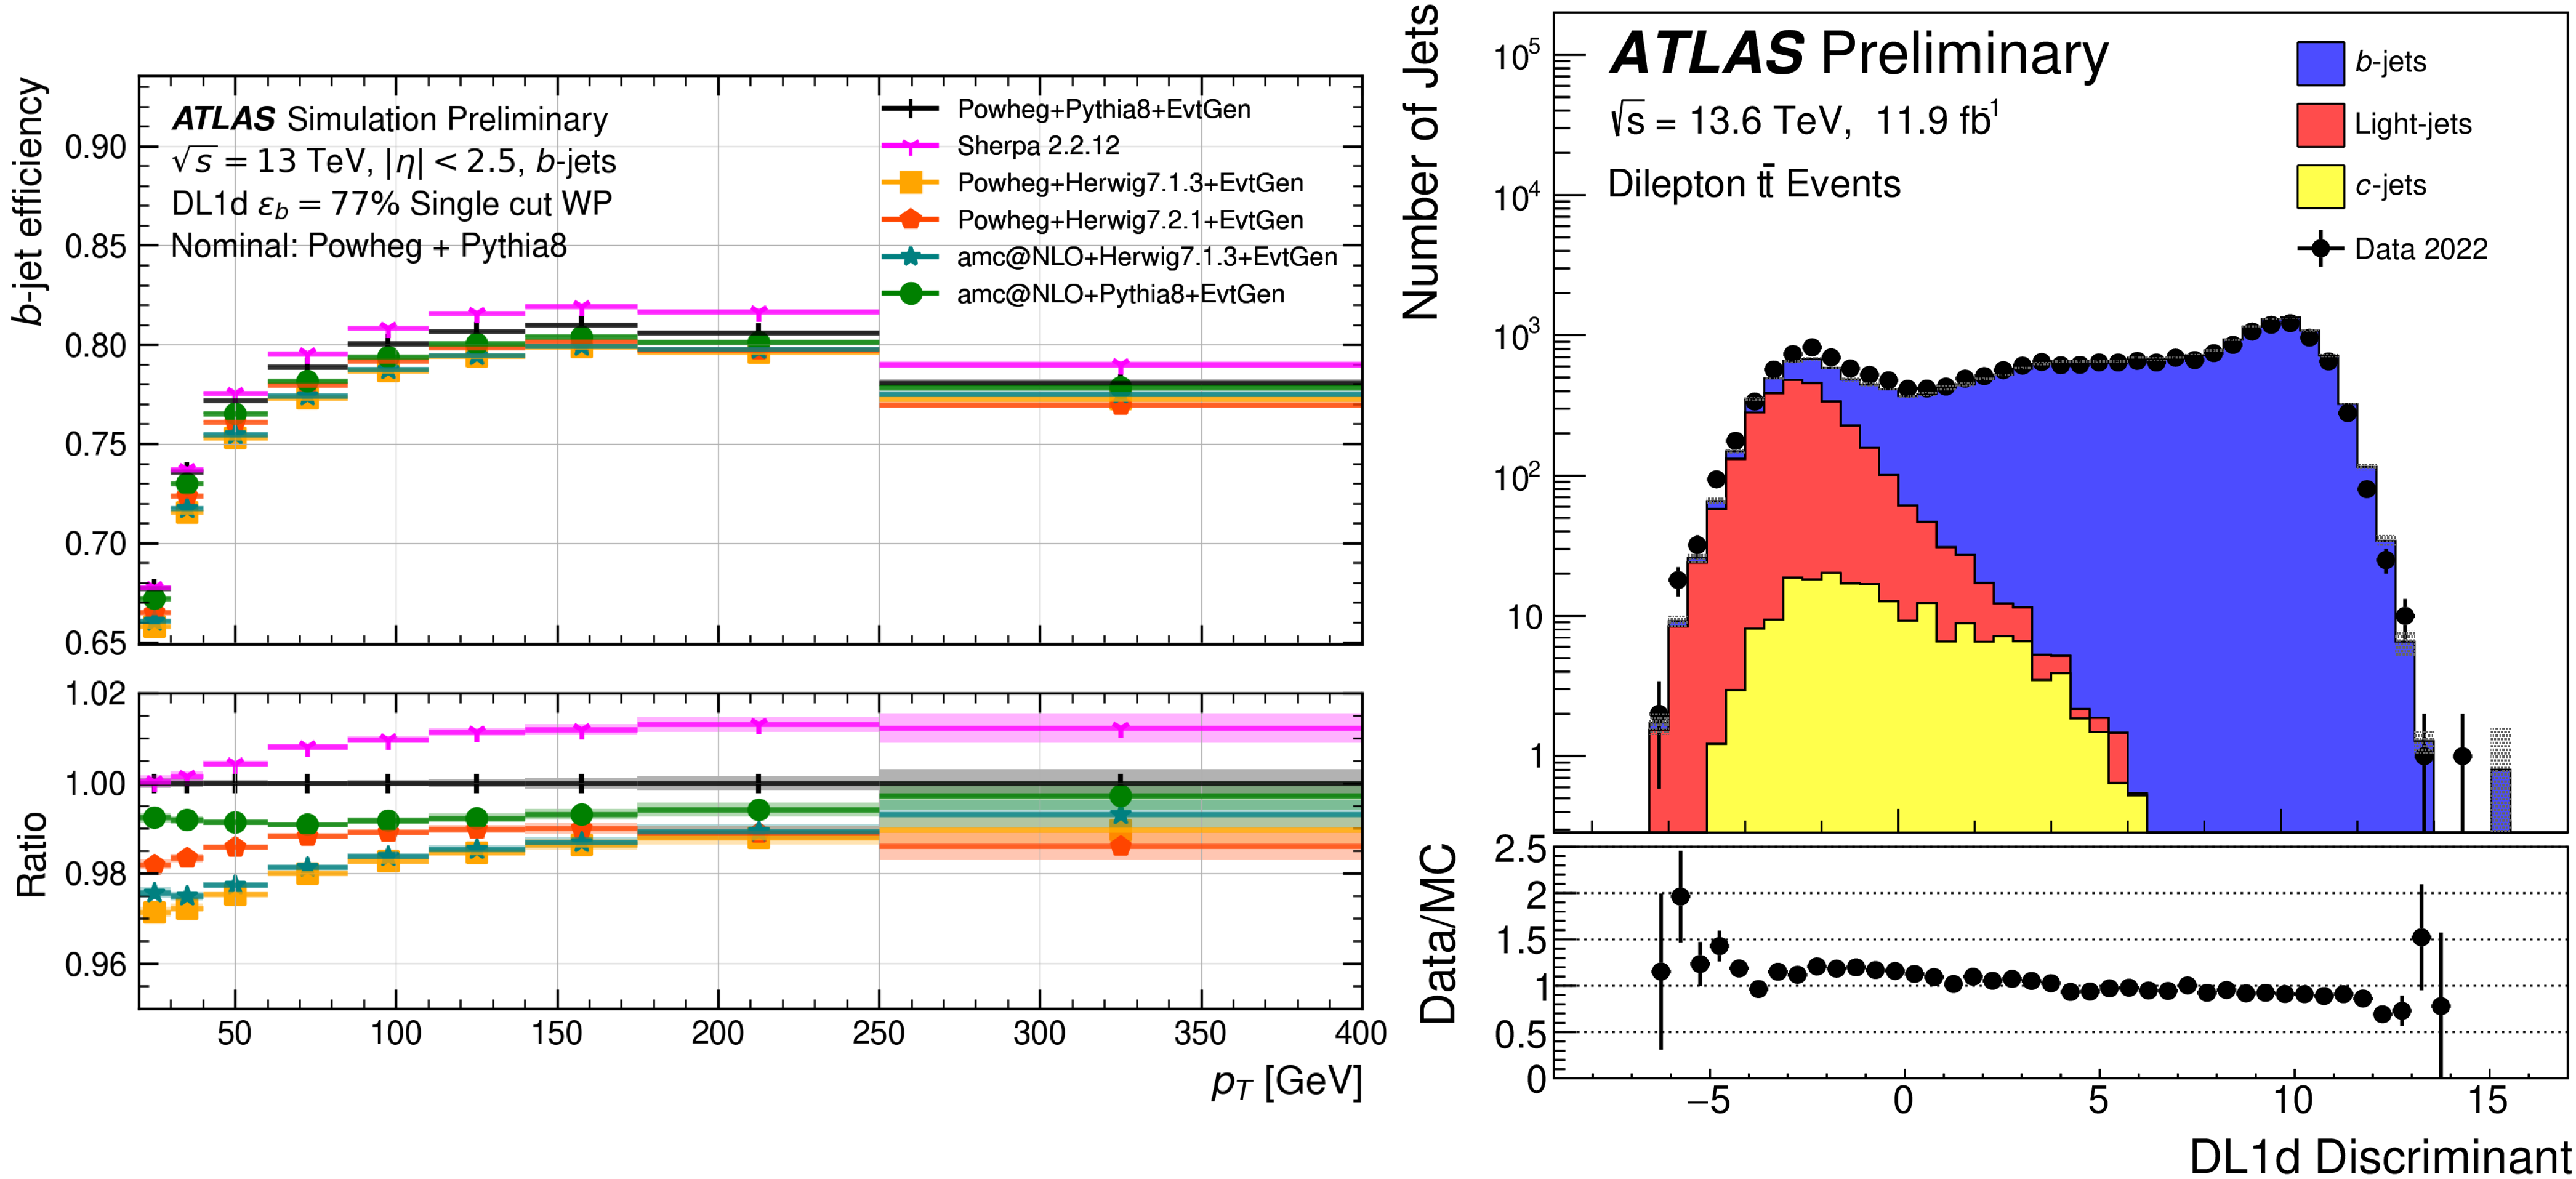
\includegraphics[width=\textwidth]{Images/FTAG/calib/sfAg.png}
  }
  \caption{Generator dependency of the $b$-efficiency as a function of jet \pt\ (left) and Data/MC agreement of the $b$-discriminant $D_b$ on a dileptonic \ttb\ Run 3 sample (right) for a calibrated DL1d $b$-jet tagger \cite{ATL-PLOT-FTAG-2023-01}. The ratio of the alternative generator to the nominal one is used to derive an MC-MC scale factor. Data-MC scale factors are derived from the Data/MC agreement of the DL1d discriminant on dedicated samples enriched in different jet species, such as the dileptonic \ttb\ process for $b$-jets. The different generators are described in Section~\ref{sec-datasets}.}
  \label{fig:calibFtagDL1d}
  \end{figure} 
\end{center}

From these studies, two types of \glspl{sf} are produced. Data-\gls{mc} \glspl{sf} are derived by comparing the output of the tagger on a simulated and real dataset using the same selection \cite{Aad:2019aic, ATLAS-CONF-2018-045, ATLAS-CONF-2018-006, cjettaggingCalib}. The efficiencies $\epsilon^f$ for each flavour $f \in {b, c, \textrm{light}}$ are measured, both on the simulated and real dataset, with \[\epsilon^f(p_T) = \frac{N^f_{\textrm{tagged}}(p_T)}{N^f_{\textrm{all}}(p_T)},\] where $N^f_{\textrm{tagged}}(p_T)$ is the number of jet of flavour $f$ in the bin of $p_T$ that are $b$-tagged and $N^f_{\textrm{all}}$ the total number of jet of flavour $f$ in the same bin. Scale factors to apply to simulations are then derived for each flavour $f$ as \[\textrm{SF}^f_{\textrm{Data-MC}}(p_T) = \frac{\epsilon^f_{\textrm{Data}}(p_T)}{\epsilon^f_{\textrm{MC}}(p_T)},\] giving the ratio of the measured efficiency in data over simulation. To include dynamics-dependent effects of the tagger, the efficiencies $\epsilon^f$ and \gls{sf} are derived in bins of jet $p_T$. Such calibration factors are applied in all analyses to correct the tagging efficiencies. This calibration is performed independently for each output flavour of the tagger, as it relies on selecting a portion of the ATLAS data with a dominating proportion of the specific flavour. The $b$-tagging efficiency is derived from a sample of $t\bar{t}$ with two charged leptons in the final state, as described in Ref. \cite{Aad:2019aic}. The \gls{sf} for $c$-jet misstagging is calibrated on a $t\bar{t}$ sample decaying to exactly one charged lepton and several jets \cite{cjettaggingCalib}. Finally, the \gls{sf} for light-jets is derived in a sample of $Z$ bosons produced in association with jets ($Z+$jets) \cite{ATLAS:2023lwk}. %Due to the extreme rejection power of modern flavour taggers, a special technique called \textit{flip tagger} is used for this last \gls{sf}, in which a tagger is modified to have a reduced light-rejection.\\

To probe the effect of different \gls{mc} simulators, \gls{mc}-\gls{mc} \glspl{sf} are derived between the chosen nominal Monte Carlo simulator used for training and alternative simulators or by changing the tuning \cite{ATL-PHYS-PUB-2020-009}. This dependency is measured by applying the same tagger to samples simulated with different generators, mainly \textsc{Pythia} \cite{SJOSTRAND2015159}, \textsc{Herwig} \cite{bellm2017herwig}, and \textsc{Sherpa} \cite{sherpa2.2paper} for variation to the parton shower and hadronisation and \textsc{MadGraph} for variation to the matrix element \cite{madgraph}. The decay chains of $b$- and $c$-hadrons in ATLAS are further simulated with the \textsc{EvtGen} package \cite{LANGE2001152}. These effects are measured into \glspl{sf} using the same technique as the data-\gls{mc} scale factors. For an alternative generator, the \glspl{sf} of flavour $f$ is derived by composing the Data-\gls{mc} \glspl{sf} with the nominal sample and the \gls{mc}-\gls{mc} \glspl{sf} as \[\textrm{SF}^f_{\textrm{Alternative}}(p_T) = \frac{\epsilon^f_{\textrm{Data}}(p_T)}{\epsilon^f_{\textrm{Nominal MC}}(p_T)} \times \frac{\epsilon^f_{\textrm{Nominal MC}}(p_T)}{\epsilon^f_{\textrm{Alternative MC}}(p_T)} = \frac{SF^f_{\textrm{data-MC}}(p_T)}{SF^f_{\textrm{MC-MC}}(p_T)}.\] These scale factors are applied in physics analyses as a per jet weight to the discriminant. Some early studies of both scale factor types have been performed in Ref. \cite{ATL-PLOT-FTAG-2023-01}, showing good agreement between the data and simulated performance of \gls{dl1d} and \gls{gn1}. Variations due to the change of generator are also found to be at most 8\% with respect to the nominal choice.

\section{Conclusion}
This chapter introduces the main machine learning models developed for heavy-flavour jet identification in ATLAS during the period covering 2020 to 2024. Work carried out in and presented in this thesis includes the first training of the \gls{dl1d} model, including the \gls{dips} sub-tagger of the first time in the ATLAS software. \gls{dl1d} is found to have improved background rejections at a fixed \gls{wp} for both $b$- and $c$-tagging compared to the at-the-time main tagger \gls{dl1r}. Excitingly, a new family of taggers based on a graph attention network for \gls{gn1} and a transformer encoder for \gls{gn2} is presented, describing the motivation and specificities behind the design. The performance of the different methods are compared, highlighting a promising increase in efficiency for the taggers developed for the Run 3 of the \gls{lhc}. Efforts to perform to optimise the hyperparameter of \gls{gn2} are introduced, addressing the possibilities of a new \gls{cern} infrastructure built on KubeFlow as well as the relevance of the maximal update parametrisation to boost the search for the best hyperparameters. 

%This chapter introduces the main machine learning models developed for heavy-flavour jet identification in ATLAS during the period covering 2020 to 2024. Work carried out in and presented in this thesis includes the first training of the \gls{dl1d} model, including the \gls{dips} sub-tagger of the first time in the ATLAS software. \gls{dl1d} is found to have improved background rejections at a fixed \gls{wp} for both $b$- and $c$-tagging compared to the at-the-time released tagger: \gls{dl1r}. Significant changes in addition to the development of this new tagger were made to the preprocessing pipeline of the \textsc{Umami} software \cite{UmamiCite} and the architecture as well as the list of features used. Finally, the new family of taggers based on graph neural network for \gls{gn1} and transformers for \gls{gn2} is presented, with the architecture adopted fully described and the performance of the different taggers compared. The hyperparameter optimisation of \gls{gn2} is also discussed, introducing the possibilities of using the new infrastructure of the KubeFlow server managed by \gls{cern} as well as the relevance of the maximal update parametrisation for improving the search for optimal hyperparameters of \gls{gn2}. Significant contributions were made to the development of the \textsc{Umami} and \textsc{Salt} software used to train the DL1 and GN families of models were made to support these studies \cite{UmamiCite, SaltCite}. 

%\begin{tcolorbox}[colback=oxfordblue!5,colframe=blue!40!black,title=Summary of the Chapter]
%In this chapter, the \gls{ftag} world is introduced. 
%\end{tcolorbox}